\section{Введение в Raft}

Алгоритм Raft подробно рассматривался в предыдущей научной работе, где были детально
разобраны его принципы, архитектура и формальные доказательства корректности. В данном
разделе будут изложены основные аспекты Raft, необходимые для понимания работы программы,
избегая избыточных деталей и сосредоточившись на ключевых механизмах протокола.

Алгоритм Raft был предложен Диего Онгаро и Джоном Оустером в 2014 году как альтернатива
Paxos, с акцентом на простоту понимания и удобство реализации. Raft предназначен для
управления реплицируемым журналом команд, обеспечивая согласованность данных в
распределённых системах.

\subsection{Основные принципы Raft}

Raft разделяет процесс достижения консенсуса на три ключевых компонента:

\begin{itemize}
    \item Выбор лидера – механизм, обеспечивающий автоматическое определение
    единственного управляющего узла (лидера) в кластере.
    \item Репликация логов – распространение команд от клиента через лидера к остальным
    узлам (последователям) с гарантией согласованности.
    \item Безопасность – гарантирует, что все узлы применяют команды в одинаковом
    порядке и не происходит разделения кластера на противоречивые группы.
\end{itemize}

Каждый узел в Raft может находиться в одном из трёх состояний:

\begin{itemize}
    \item Лидер (Leader) – единственный узел, обрабатывающий запросы от клиентов и
    координирующий репликацию логов.
    \item Последователь – пассивный узел, принимающий команды от лидера и подтверждающий
    их выполнение.
    \item Кандидат – узел, инициирующий процесс выборов в случае отсутствия лидера.
\end{itemize}

\subsection{Выбор лидера}

Выбор лидера происходит, когда существующий лидер становится недоступным. Последователи
инициируют выборы, переходя в состояние кандидатов и отправляя запросы голосования
(RequestVote) остальным узлам. Каждый узел голосует только один раз в одном терминальном
периоде (\textit{term}), а кандидат, получивший большинство голосов, становится новым
лидером.  

Чтобы избежать сплит-голоcования, Raft использует случайные таймеры выборов. Это
минимизирует вероятность одновременного запуска выборов несколькими узлами.

\subsection{Репликация логов}

Одной из ключевых задач алгоритма Raft является обеспечение согласованности логов между
узлами кластера. Для этого используется механизм репликации записей, который гарантирует,
что все узлы имеют одинаковую последовательность команд, применяемых к их состоянию.

\begin{figure}
  \centering
  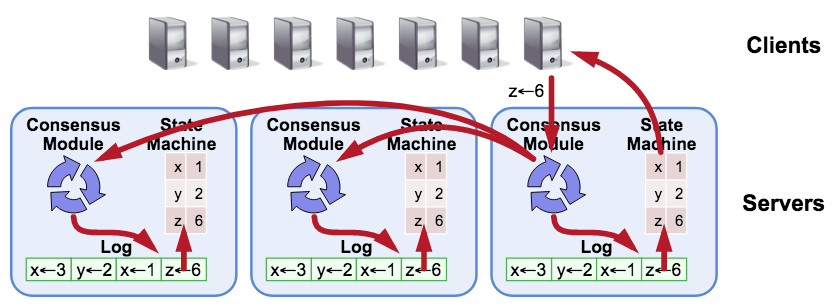
\includegraphics[scale=0.6]{assets/raft_replication.png}
  \caption{Механизм репликации логов в алгоритме Raft}
  \label{fig:raft-replication}
\end{figure}

Процесс репликации логов показаны на рисунке~\ref{fig:raft_replication}. Клиент
отправляет запрос на изменение состояния в кластер, который обрабатывает текущий лидер.
Лидер добавляет новую запись в свой лог и рассылает её последователям с помощью
сообщений \texttt{AppendEntries}. Узлы последовательно добавляют полученные команды в
свои журналы, сохраняя порядок операций. Как только большинство узлов подтверждает запись
, она считается зафиксированной, после чего команды могут быть применены к конечному
автомату каждого узла.

\subsection{Механизм безопасности}

Raft строго гарантирует, что ни один узел не применит команду до её репликации на
большинстве узлов. Кроме того, протокол предотвращает ситуацию, когда новый лидер может
иметь устаревшие данные:

\begin{itemize}
    \item Кандидат должен содержать все подтверждённые записи, иначе он не сможет
    выиграть выборы.
    \item Узлы отклоняют запросы от лидера, если у него устаревший термин.
    \item Если новый лидер обнаруживает конфликтующие записи у последовательных узлов,
    он удаляет их и заново отправляет правильные данные.
\end{itemize}

Эти механизмы позволяют Raft поддерживать строгую согласованность даже в случае сбоев.

\subsection{Изменение состава кластера}

Raft поддерживает безопасное добавление и удаление узлов с помощью механизма
\textit{joint consensus}. В этом режиме временно существуют два пересекающихся кворума
(старый и новый состав), что гарантирует плавный переход и предотвращает разделение
кластера.
